\section{Real World Configuration}
\label{sec:realWorld_description}

Files are provided to run real-world simulations with realistic topography, wind forcing, and temperature and salinity restoring.  
Most of the horizontal grids are quasi-uniform over the globe, with simulations performed at nominal grid cell widths of 240, 120, 60, 30, and 15 km.  These grids are based on Voronoi tessellations with uniform grid density, which results in grid that is almost all hexagons.  An additional grid file is provided for a variable resolution simulation that has 15 km gridcells in the North Atlantic and 75 km gridcells elsewhere, with a smooth transition in between \citep[Figure 2]{Ringler_ea13om}.

Initial distributions of potential temperature and salinity are obtained from the annual mean WOCE climatology \citep{Gouretski:2004wv}.  Initial velocities are zero, and the simulations are spun up for ten years using a constant wind stress obtained from "Normal Year" forcing data from the Coordinated Ocean Reference Experiment (CORE, \citet{Large:2004ug}), and surface temperature and salinity are restored to the initial condition with a time scale of 30 days.  

Simulations are similar to those presented in \citet{Ringler_ea13om}, and include the following: z-star vertical coordinate with 40 vertical layers, ranging in thickness from 10 m near the surface to 250 m in the deep ocean; quadratic bottom drag with a coefficient of 0.01; nonlinear equation of state by \citet{Jackett_McDougall95jaot}; monotonic flux-corrected tracer transport \citep{Skamarock_Gassmann11jcp}, with third order reconstruction of the tracer values at the cell edges.  The horizontal turbulence closure is a simple hyperviscosity ($-\nabla^4$) operator with coefficients of $\nu_h = \nu_0 (\Delta x / \Delta x_0)^3$ with $\nu_0=5\times10^{10}$ and $\Delta x_0=15$ km grid cells.  Zero horizontal diffusion is applied to the tracers.  The vertical mixing is Richardson number-based, with background viscosity and diffusion of $10^{-4}$ and $10^{-5}$ m$^2$ s$^{-1}$, respectively.


\subsection{Provided Files}
\label{subsec:realWorld_files}

\begin{itemize}
	\item ocean\_QU\_15km.nc, ocean\_NA\_15km\_75km.nc, etc: \\
		These are the input grid files that include conditions after the initial ten year spin-up. They can be visualized in the same way output files can to see the initial conditions. File names indicate a quasi-uniform mesh (QU) or North Atlantic variable resolution mesh (NA), and the nominal grid cell size is specified.
	\item graph.info: \\
		This file is a graph of all of the cells in the mesh. \\
		It is used to decompose the mesh into partition files.
	\item graph.info.part.$n$: \\
		This is a partition file for use with an $n$ processor run, where $n$ is a typical number for the given resolution.  For example, the 240 km mesh may be run on 1 to 16 processors, while the 15 km requires thousands of processors.
	\item namelist.input: \\
		This is the namelist file with all parameters for the run. \\
		It has a default setup which when run provides the results in the next section.
\end{itemize}

\subsection{Results}
\label{subsecc:realWorld_results}

The simulations were run for one year using the provided files, and visualized using Paraview (see Chapter \ref{chap:mpas_visualization}).

\begin{figure}[H!]
	\centering
(a)	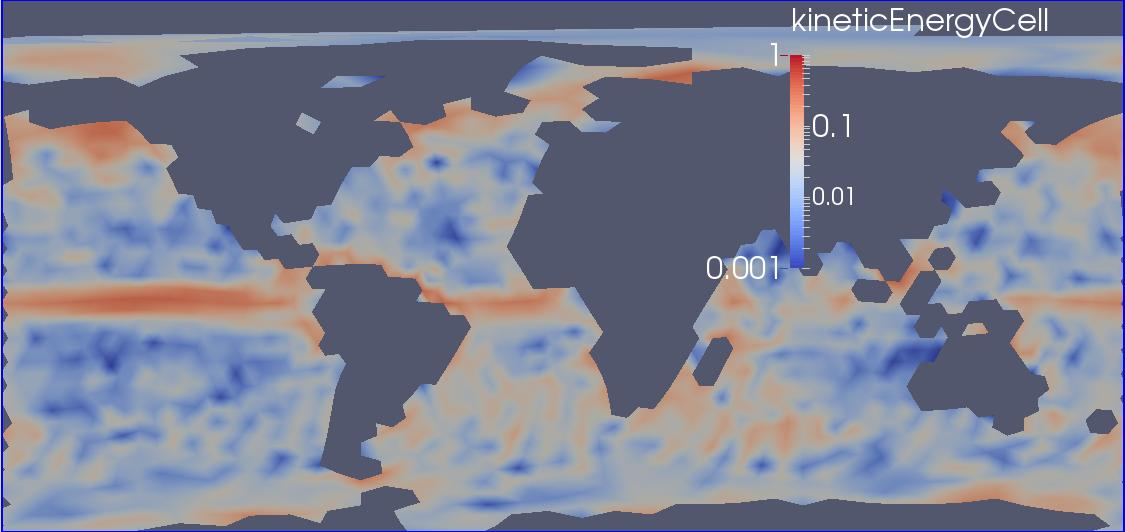
\includegraphics[scale=0.36]{ocean/figures/m72m_240km_yr11_k1_ke.jpg}\\
%	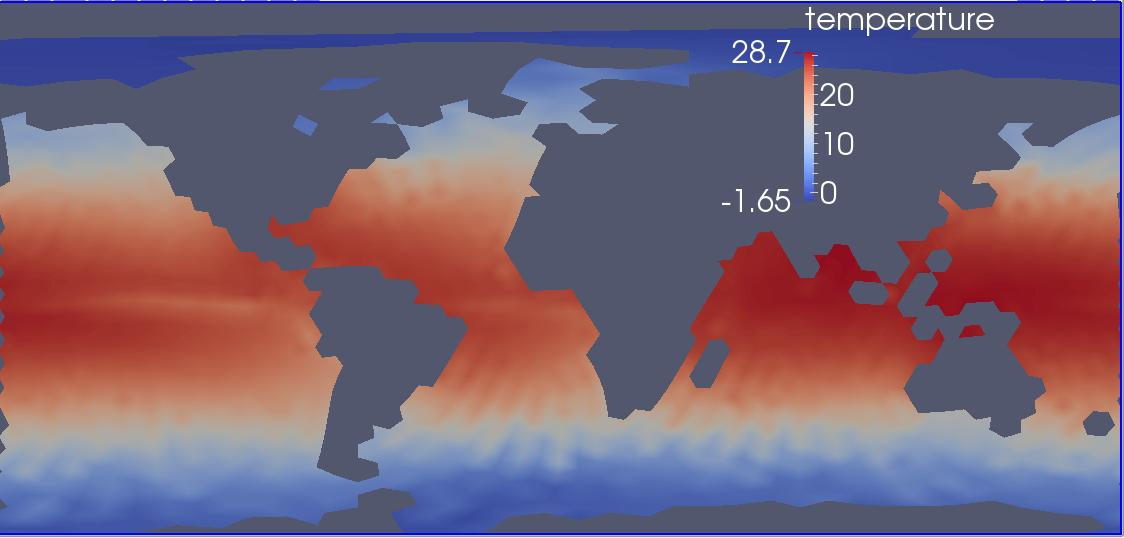
\includegraphics[scale=0.18]{ocean/figures/m72m_240km_yr11_k1_T.jpg}
(b)	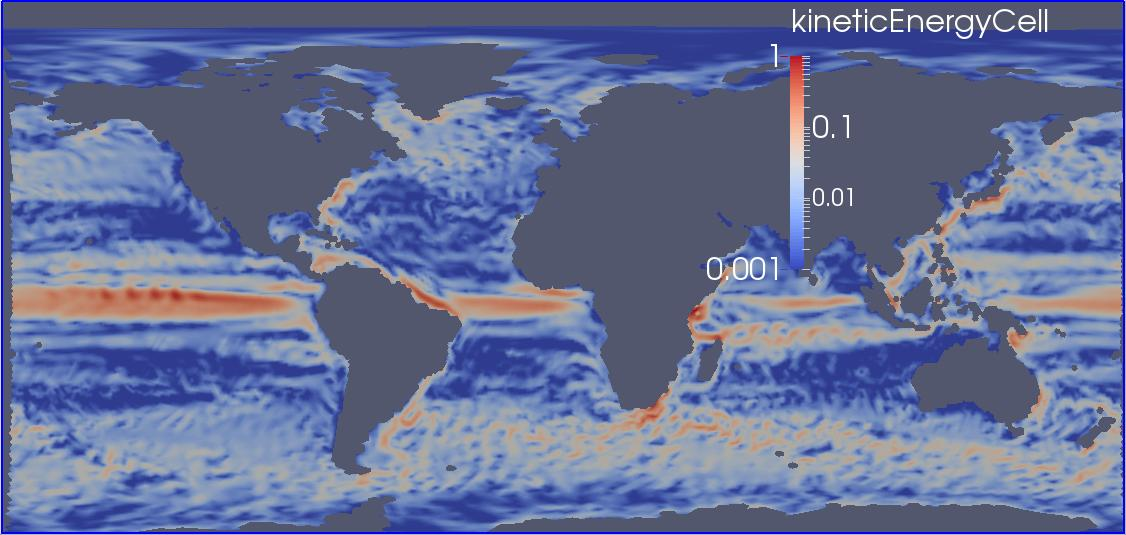
\includegraphics[scale=0.36]{ocean/figures/m72g_120km_yr11_k1_ke.jpg}\\
%	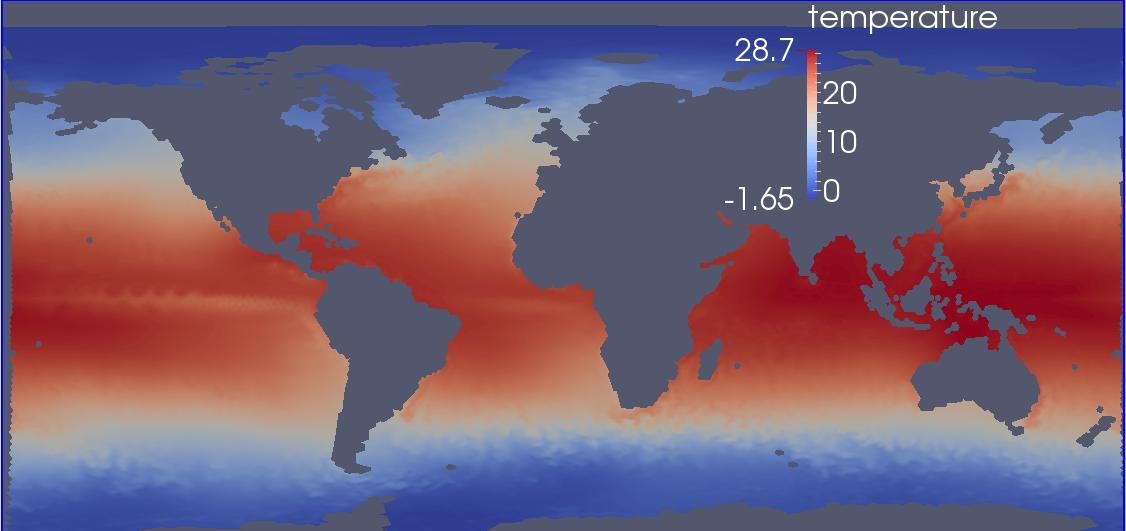
\includegraphics[scale=0.18]{ocean/figures/m72g_120km_yr11_k1_T.jpg}\\
(c)	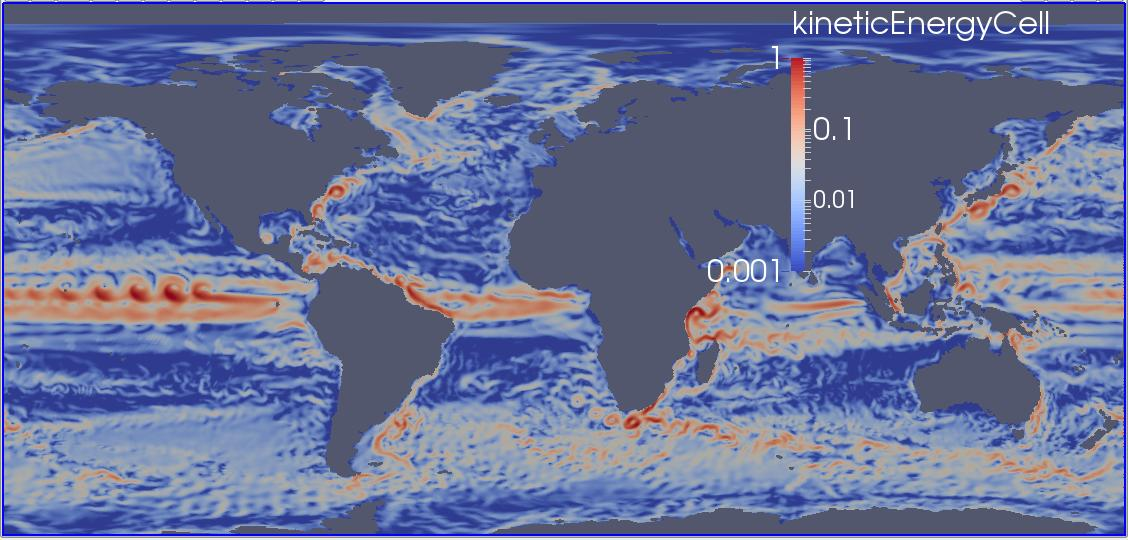
\includegraphics[scale=0.36]{ocean/figures/m72h_60km_yr11_k1_ke.jpg}
%	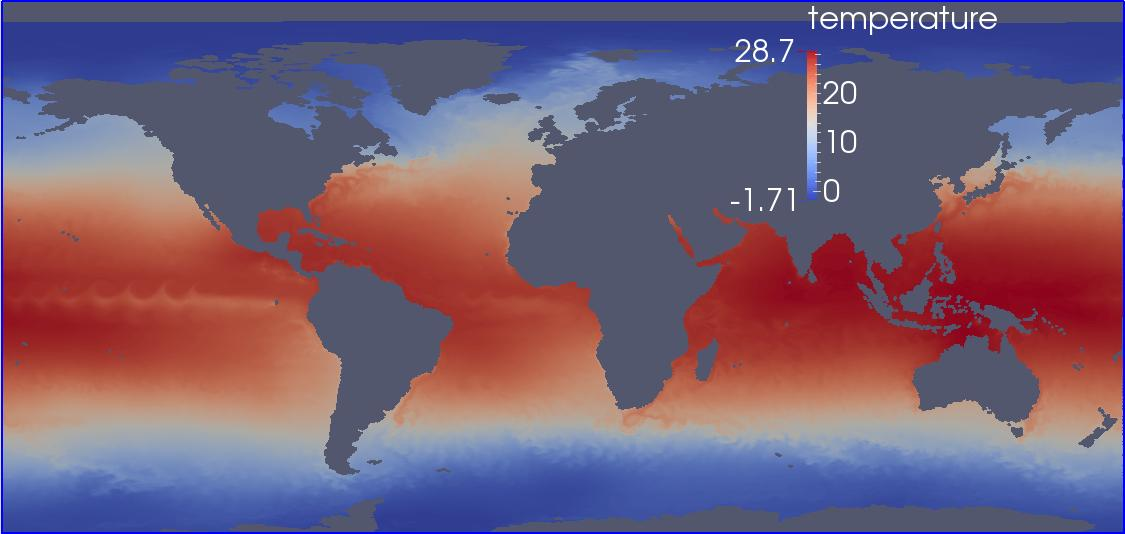
\includegraphics[scale=0.18]{ocean/figures/m72h_60km_yr11_k1_T.jpg}\\
%(d)	\includegraphics[scale=0.18]{ocean/figures/m72i_30km_yr11_k1_ke.jpg}
%	\includegraphics[scale=0.18]{ocean/figures/m72i_30km_yr11_k1_T.jpg}\\
%(e)	\includegraphics[scale=0.18]{ocean/figures/m72k_15km_yr6_k1_ke.jpg}
%	\includegraphics[scale=0.18]{ocean/figures/m72k_15km_yr6_k1_T.jpg}\\
%(f)	\includegraphics[scale=0.18]{ocean/figures/m72j_NA_15km_yr11_k1_ke.jpg}
%	\includegraphics[scale=0.18]{ocean/figures/m72j_NA_15km_yr11_k1_T.jpg}
	\caption{Kinetic energy in m$^2$ s$^{-2}$ at the surface for real world test cases.  Resolutions increase from top to bottom with: (a) 240 km, (b) 120 km, (c) 60 km} %, (d) 30 km, (e) 15 km, all quasi-uniform, and (f) variable resolution North Atlantic 15 km. }
	\label{fig:overflow}
\end{figure}

